\documentclass[12pt]{article}
\usepackage[a4paper,margin=1in,footskip=0.25in]{geometry} % set margins
\usepackage[portuguese]{babel}
\usepackage[utf8]{inputenc}
\usepackage{hyperref} 
\usepackage{amsmath}
\usepackage{amssymb}
\usepackage{amsthm}
\usepackage{graphicx}    % needed for include graphics
\usepackage{indentfirst}
\usepackage{float}       % needed for [H] figure placement option
\usepackage{setspace}    % needed for doublespacing
\usepackage{tikz}

% Macros
\renewcommand{\familydefault}{\sfdefault} % sans-serif
\newcommand{\lowtext}[1]{$_{\text{#1}}$}

% Adds ./figures/ to the path of figures
\graphicspath{./figures/}

\title{Arquitetura do Console Nintendo 64}
\author{Antonio Augusto Abello, Gustavo Estrela de Matos, Lucas Romão
Silva}

\begin{document}
% Espaçamento duplo 
\doublespacing
\begin{titlepage}
    \vfill
    \begin{center}
        \vspace{0.5\textheight}
        \noindent
        Instituto de Matemática e Estatística \\
        Monografia dos curso Organização de Computadores \\
        \vfill
        \noindent
        {\Large Arquitetura do Console Nintendo 64} \\
        \begin{tabular}{rl}
            {\bf Professor:} & {Siang Wun Song} \\
            {\bf Alunos:}    & {Antonio Augusto Abello} \\
                             & {Gustavo Estrela de Matos} \\
                             & {Lucas Romão Silva} \\
        \end{tabular} \\
        \vspace{\fill}
       \bigskip
        São Paulo, \today \\
       \bigskip
    \end{center}
\end{titlepage}

\pagebreak
\tableofcontents
\pagebreak

\section{Introdução}
No seguinte trabalho buscamos explicar o funcionamento do console de Nintendo 64 do ponto de vista da Organização de Computadores. Queríamos também, como objetivo secundário, entender como esse funcionamento pode ser eventualmente emulado por software em outras arquiteturas e dispositivos.
Para tanto fazemos primeiro uma exposição da arquitetura geral, seguida de outras sobre os principais componentes do dispositivo, visando sempre explicar sua integração e seu funcionamento no contexto mais geral. Ao fim temos uma parte sobre como se dá a emulação desses processos que funciona como conclusão do artigo. No fim do trabalho também se encontram as referências utilizadas na pesquisa.
\section{Arquitetura Geral}

O Nintendo 64 consiste em um conjunto de componentes de hardware que
trabalham em conjunto para o processamento gŕafico e de áudio. O componente
chave do sistema é o RCP, que faz a conexão com todos os outros componentes, a memória, e as entradas e saídas do sistema (Áudio, Vídeo, Input). A CPU e o RCP rodam concorrentemente; na CPU, os processos são rodados em \textit{threads} ao passo em que no RCP os processos são rodados em
\textit{tasks}.

Na CPU, os processos rodam no conjunto de \textit{threads} onde cada uma
possui sua própria pilha de execução. Diferentemente dos sistemas UNIX,
no console não existe o conceito de relógio de swap ou de
\textit{round-robin} para o escalonamento, isto é, uma \textit{thread}
que possui CPU não é interrompida, caso exista outra de mesma prioridade
a CPU só será removida da mesma quando ela acabar sua execução ou caso
outra \textit{thread} de maior prioridade.

\begin{figure}[H]
    \label{fig:block-diagram}
    \centering
        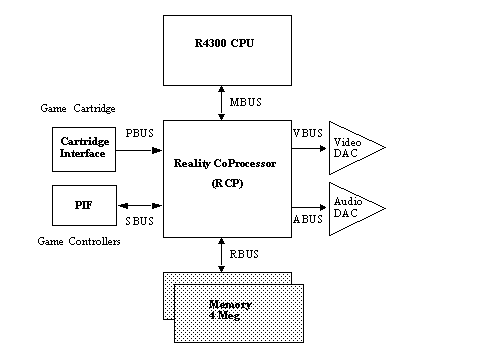
\includegraphics[scale=.65]{figures/nintendo64-diagram}
    \caption{Diagrama de blocos do hardware do Nintendo 64}
\end{figure}

No aspecto do software, o sistema operacional do Nintendo 64 é responsável pela tradução de
funções lógicas e argumentos para as configurações específicas
do hardware, enquanto boa parte do gerenciamento dos recursos
é deixada para os jogos. As únicas interfaces já fornecidas prontas
pelo console são a de E/S e de áudio.

Nas seções que seguem, será falado mais a fundo sobre os componentes do
console e suas respectivas funções no processamento de um jogo.


\section{Chip NEC VR4300}
    O chip NEC VR4300 é o principal processador no Nintendo64,
responsável principalmente por processar a lógica dos jogos e, 
também audio. Esse processador foi desenvolvido pela empresa japonesa
NEC e implementa a arquitetura de conjunto de instruções MIPS, 
desenvolvida pela empresa de mesmo nome. A arquitetura MIPS define um
conjunto de instruções do tipo RISC, \emph{reduced instruction set
computer}.

    O processador VR4300 possuia uma arquitetura compatível com 
instruções de 64 bits, apesar de grande parte das instruções do
Nintendo 64 serem de apenas 32 bits. Especificamente nesse console, o
processador da NEC trabalhava a uma frenquência de 93,75 MHz.

\subsection{Principais Componentes do Processador VR4300}
    A figura \ref{fig:vr4300dia} mostra um diagrama com os principais
componentes do processador VR4300 e como eles se comunicam. Nesta seção,
discutiremos o papel de cada um desses componentes.
\begin{itemize}
    \item {\bf System interface} define a interface do chip com os
componentes externos. Essa interface é formada por um bus de 32 bits
e vários outros bits para controle de bits, interrupções, relógio, etc.
No Nintendo  64, algum desses bits se conectam a memória RAM do console
e, também diretamente ao cartucho com o jogo.
    \item {\bf Clock generator} é responsável por determinar o clock
interno do chip, que é o clock do pipeline do processador. Esse 
componente recebe um clock externo e define o clock de pipeline como uma
fração do anterior. Um dos modos de operação do VR4300 é ter o relógio 
interno funcionando com 2 ciclos a cada ciclo do relógio externo.
    \item {\bf Instruction cache} é um cache que guarda a instrução que
está sendo executada. No contexto do pipeline, manter uma cópia da 
instrução lida dentro do processador é essencial para aumentar 
eficiência e permitir operações como desvios e interrupções.
    \item {\bf Execution unit} é uma parte do hardware que é 
especializada em realizar operações aritméticas. Na arquitetura MIPS,
a {\em Execution unit} tem o papel de {\em COP1} (coprocessador 1).
    \item {\bf CP0} é o componente responsável por fazer o controle da
memória (MMU), isto é, permite enderaçemento virtual, controla o acesso
a pedaços de memória diferentes, aloca páginas de memória e outras 
funções. Para ajudar na eficiência de acesso a memória, o {\em} CP0 
possui uma {\em TLB} ({\em Translation Lookaside Buffer}) que é, 
basicamente, um cache para a tradução de endereços virtuais para 
físicos.
    \item {\bf Data cache} é um cache para dados da memória. Os dados 
armazenados nesse componente são indexados pelos endereços virtuais.
Podemos ver, no diagrama, uma conexão entre {\em Execution Unit} e esse 
componente, essa ligação é utilizada quando um dado necessário em uma
computação já está no cache. Quando isso acontece poupamos o trabalho
de buscar dados na memória ou qualquer outro componente pois ele já
está disponível dentro do chip.
    \item {\bf Instruction address} tem o papel de calcular o endereço
da próxima instrução. Esse circuito deve ser capaz de incrementar o
{\em Program Counter}, dando sequência as execuções de instruções, e
também deve ser capaz de atualizar o {\em Program Counter} quando
ocorrem desvios ({\em branch} e {\em jump}).
    \item {\bf Pipeline control} é o circuito que controla a execução
do pipeline do processador. O conceito de pipeline consiste em dividir
a execução de uma tarefa de maneira que mais de uma tarefa possa ser
executada simultaneamente, desde que em diferentes etapas e não 
dependentes. O pipeline do processador VR4300 consiste em cinco etapas
diferentes:
    \begin{itemize}
        \item{IC (Instruction Cache Fetch):} faz a leitura da instrução.
        \item{RF (Register Fetch):} deixa valores de registradores 
prontos para serem usados em cálculos.
        \item{EX (Execution):} executa operações aritméticas.
        \item{DC (Data Cache Fetch):} armazena no cache os dados 
utilizados na instrução.
        \item{WB (Write Back):} atualiza valores na memória ou 
registradores.
    \end{itemize}
O que ocorre em cada etapa do pipeline também depende muito da instrução
que está sendo executada, portanto o que está descrito logo acima é uma
visão superficial de cada uma dessas etapas.
\end{itemize}

\begin{figure}[H]
    \label{fig:vr4300dia}
    \centering
       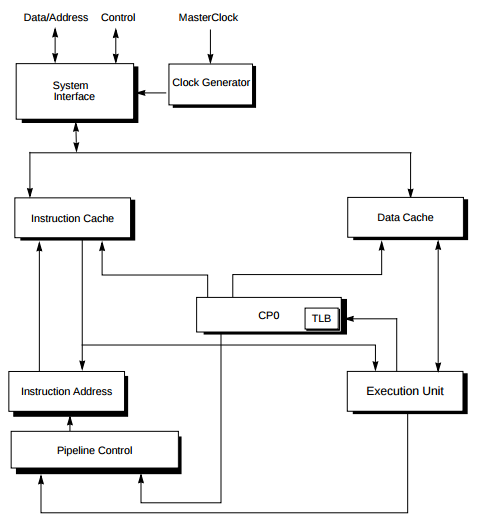
\includegraphics[scale=.65]{figures/vr4300diagram}
    \caption{Um diagrama com os principais componentes do processador 
        VR4300}
\end{figure}

\subsection{Formato de instrução}
    Cada instrução do processador é formada por 32 bits, e elas podem
ser separadas em três categorias: \emph{I-type}, \emph{J-Type} e 
\emph{R-Type}. 

    As intruções do tipo \emph{I-Type} são formadas por 5 bits, $op$,
que determinam a operação; 5 bits em $rs$ e mais 5 em $rt$, que
determinam os registradores que estão sendo operados; e mais 16 bits,
{\em immediate}, que pode representar ou um enderço ou uma constante.
Exemplos de instruções desse tipo são as instruções {\em load} e 
{\em store}.

\begin{figure}[H]
\centering
\begin{tikzpicture}[>=latex, font=\sffamily, every node/.style = 
     {minimum height = 1.5em, outer sep = 0pt, 
     draw=black, fill = blue!20,semithick}]
        \node [minimum width=2cm] 
            at (0,0)    (A) {op};
        \node [anchor=west, minimum width=2cm] 
            at (A.east) (B) {rs};
        \node [anchor=west, minimum width=2cm] 
            at (B.east) (C) {rt};
        \node [anchor=west, minimum width=6cm] 
            at (C.east) (D) {immediate};
        \node [draw=none, fill=none, anchor=west, 
                xshift=2.5cm, yshift=0.75em] 
            at (D.north) (D) {0};
        \node [draw=none, fill=none, anchor=west, 
                xshift=0.25cm, yshift=0.75em] 
            at (C.north) (D) {16};
        \node [draw=none, fill=none, anchor=west, 
                xshift=0.25cm, yshift=0.75em] 
            at (B.north) (D) {21};
        \node [draw=none, fill=none, anchor=west,
                xshift=0.25cm, yshift=0.75em] 
            at (A.north) (D) {26};
        \node [draw=none, fill=none, anchor=west,
                xshift= -1.25cm, yshift=0.75em] 
            at (A.north) (D) {31};
\end{tikzpicture}
\caption{Formato de uma instrução \em{I-Type}} 
\label{fig:instr-itype}
\end{figure}

    As intruções do tipo {\em J-Type} são usadas para controlar o fluxo
do programa. Para isso, esse tipo de instrução pode pular para um 
pedaço específico do código por via de um {\em jump} ou um {\em branch}.
Quando uma instrução do tipo {\em jump} é executada, o desvio sempre 
acontece, ao contrário da instrução {\em branch} na qual é possível 
determinar uma condição para o desvio. No VR4300 essas intruções são
formadas por 5 bits, $op$, que determinam a operação; e mais 26 bits
$target$, que determinam o endereço do possível desvio. Quando a 
instrução é um desvio obrigatório, os 26 bits estão todos disponíveis
para determinar o endereço de destino, mas no caso de um {\em branch}
o valor de $target$ só pode determinar um {\em offset} de 16 bits 
relativo ao registrador {\em PC}.

\begin{figure}[H]
\centering
\begin{tikzpicture}[>=latex, font=\sffamily, every node/.style = 
     {minimum height = 1.5em, outer sep = 0pt, 
     draw=black, fill = blue!20,semithick}]
        \node [minimum width=2cm] 
            at (0,0)    (A) {op};
        \node [anchor=west, minimum width=10cm] 
            at (A.east) (B) {target};
        \node [draw=none, fill=none, anchor=west, 
                xshift=4.75cm, yshift=0.75em] 
            at (B.north) (B) {0};
        \node [draw=none, fill=none, anchor=west, 
                xshift=0.25cm, yshift=0.75em] 
            at (A.north) (A) {26};
\end{tikzpicture}
\caption{Formato de uma instrução \em{J-Type}} \label{fig:instr-jtype}
\end{figure}

    As instruções do tipo {\em R-Type} envolvem apenas o uso de 
registradores. Exemplos de instruções desse tipo são aquelas que
fazem operações aritméticas entre dois registradores e guardam o 
resultado em um terceiro registrador. Essas instruções são formadas
por 5 bits $op$; 5 bits para cada um dos três registradores $rs$, $rt$
e $rd$; 5 bits $sa$ que definem um {\em shift} para o resultado; e mais
6 bits para $function$.

\begin{table}[H]
\centering
\label{r-type-table}
\begin{tabular}{|c|c|}
\hline
Code & Operation \\ \hline
0  & Add \\
1  & Subtract \\
2  & Multiply \\
3  & Divide \\
4  & Square root \\
5  & Absolute value \\
6  & Transfer \\
7  & Sign reverse \\
8  & Convert to 64-bit fixed-point, rounded to nearest/even \\
9  & Convert to 64-bit fixed-point, rounded toward zero \\
10 & Convert to 64-bit fixed-point, rounded to + $\infty$ \\
11 & Convert to 64-bit fixed-point, rounded to – $\infty$ \\
12 & Convert to 32-bit fixed-point, rounded to nearest/even \\
13 & Convert to 32-bit fixed-point, rounded toward zero \\
14 & Convert to 32-bit fixed-point, rounded to + $\infty$ \\
15 & Convert to 32-bit fixed-point, rounded to – $\infty$ \\
16–31 & Reserved \\
32 & Convert to single floating-point \\
33 & Convert to double floating-point \\
34 & Reserved \\
35 & Reserved \\
36 & Convert to 32-bit fixed-point \\
37 & Convert to 64-bit fixed-point \\
38–47 & Reserved \\
8–63 & Floating-point compare \\
\hline
\end{tabular}
\caption{Lista de todas as possíveis funções em uma instrução do tipo
{\em R-Type} \cite{vr4300-datasheet}.}

\end{table}


\section{Reality Coprocessor (RCP)}
O chip RCP (Reality Coprocessor) é, na verdade, uma coleção de processadores, interfaces de memória e lógica de E/S
Seus dois processadores são o RSP (Reality Signal Processor) e o RDP (Reality Display Processor). Ambos possuem responsabilidades parecidas (cuidam de partes distintas do processo de geração de imagem e o RSP cuida sozinho do áudio) e são separados para aumentar a performance do sistema ao realizar suas tarefas em paralelo.
A parte de E/S coneceta o RCP com a CPU, os inputs, o cartucho e também possui saídas \textit{write-only} de áudio e vídeo. Essas conexões são necessárias porque a parte mais lógica do processamento de áudio e vídeo é feita pela CPU
A figura abaixo mostra um esquema dos componentes do RCP.

\begin{figure}{H}
\centering
        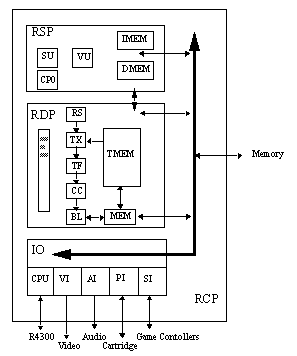
\includegraphics[scale=.65]{figures/RCP_general}
    \caption{Um diagrama com os principais componentes do co-processador RCP}
\end{figure}

\subsection{RSP}

O RSP ( \textit{Reality Signal Processor} ) é um processador que se 
especializa na execução das transformações
geométricas além de fornecer visibilidade para as funcionalidades do RCP.

Outra função também realizada pelo RSP é executar a decodificação do áudio,
apesar de este procedimento também poder ser feito pela CPU.
Dentre os consoles da época, o Nintendo 64 era o único que não possuía um
chip dedicado ao processamento de áudio, cabendo então ao programador
decidir se o processamento do áudio seria feito na CPU ou no RSP.
Por um lado, isso permitia que o sistema fosse flexível às necessidades de
cada jogo, por outro lado, isso exigia que o programador soubesse usar
corretamente as funcionalidades do console a fim de melhorar a performance
do console.

O RSP é totalmente reprogramável através do microcódigo ($\mu$code). Através
deste, era possível adicionar novas funcionalidades, novas operações
geométricas, novos efeitos além de otimizações para velocidade ou qualidade
de processamento. Entretanto, o acesso ao $\mu$code só foi liberado pela
Nintendo no final do ciclo de vida do console.

\textbf{Unidades de processamento do RSP}

\begin{itemize}
    \item Scalar Unity (SU): Usa um subconjunto de R4000 instruções para execução
    \item Vector Unity (VU): possui mecanismos para operação soma-produto de 16 bits
    \item Instruction Memory (IMEM): Memória que armazena o microcódigo
    \item Data Memory (DMEM): Espaço de memória usado pelo microcódigo
\end{itemize}




\subsection{RDP}
O RDP é um processador que se especializa na parte final de processamento de vídeo, possuindo diversos componentes para realizar essa tarefa. Recebe a maioria de suas informações e instruções do RSP, mas também ocasionalmente recebe instruções via código para alterar seu modo de execução. Conta ainda com uma memória específica para guardar texturas (TMEM) de 4KB e ao final de seu pipeline escreve na memória (na parte reservada ao \textit{framebuffer} os pixels prontos. Ele possui 6 blocos lógicos (que em hardware são implementados como vários blocos, mas agem como um só)
\begin{itemize}
    \item{Rasterizador (RS): rasteriza triângulos e retângulos}
    \item{Unidade de Textura (TX): realiza \textit{sample} das texturas carregadas em TMEM}
    \item{Unidade de Filtro de Textura (TF): filtra os \textit{samples} de textura}
    \item{Combinador de Cor (CC): interpola e combina duas cores (por exemplo, da textura e da iluminação)}
    \item{Blender (BL): mistura os pixels gerados com os pixels atuais no buffer (para transição), realiza operações relacionadas à profundidade (\textit{z-buffer}) para produzir o 3D e o \textit{anti-aliasing} (redução de serrilhados}
    \item{Interface de Memória (MI): realiza as operações de leitura, escrita e modificação dos pixels um a um no \textit{framebuffer} (em 1 ou 0.5 pixel-por-clock). Também carrega a TMEM usando os endereços físicos e lê/escreve o \textit{z-buffer}}
\end{itemize}

\section{Interface de Vídeo}
Ao final de todo o processamento da CPU, RSP, RDP, a interface de vídeo lê o \textit{framebuffer} e gera os sinais RGB, podendo trabalhar tanto em PAL ou NTSC. Ela ainda realiza um segundo passo do algoritmo \textit{anti-alias} e pode alterar a escala das imagens.
O processamento de imagens, então, passa por quase todo hardware, começando na CPU, com a parte mais lógica, passando ao RSP com a geometria e terminando no RDP com a renderização, texturização e finalização

\begin{figure}[H]
    \centering
        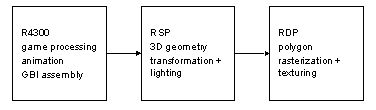
\includegraphics{figures/Video_pipeline}
    \caption{Esquema geral de processamento de vídeo}
\end{figure}

\section{Emulação}
O processo de emulação do hardware do Nintendo 64 é relativamente simples.
 Usando da capacidade de abstração provida pela programação orientada a objetos, pode-se modelar cada pedaço do hardware como um objeto ou uma estrutura (struct) e depois programar a interação entre eles como as ligações reais. Os projetos tendem também a ser altamente modularizados, sendo que em geral o emulador em si refere-se à emulação da CPU e os outros aspectos (RSP, RDP/Vídeo, Áudio, Controle) são adicionados como plug-ins programados por terceiros. 
 
A emulação da CPU é geralmente mais direta, implementando os componentes explícitamente (até coisas como TLB, memória, etc). Isso é possível somente porque os computadores atuais são poderosos o suficiente e o Nintendo 64 é simples o suficiente para essa estratégia ser efetiva. Em tempos anteriores, com computadores menos potentes, uma estratégia de emulação mais abstrata (HLE - High Level Emulation) era utilizada: se implementava as chamadas que os jogos faziam como uma livraria em C\cite{HLE}.Para sistemas mais modernos e complexos, uma estratégia semelhante deve ser utilizada. Além disso, quanto à leitura, interpretação, e execução dos códigos três estratégias distintas podem ser utilizadas 
\begin{itemize}
\item{Interpretador}: interpreta os comandos no momento em que são necessários
\item{Recompilador dinâmico}: compila um bloco de comandos de cada vez, geralmente parando em um condicional.
\item{Recompilador estático}: teóricamente seria possível usar a estratégia anterior para compilar o jogo inteiro de uma vez. No entanto isso é computacionalmente complicado e, em algumas instâncias corresponde ao problema de parada.
\end{itemize}

Diferentes problemas aparecem no contexto do desenvolvimento dos plugins. Aqui, a abstração do hardware real em uma emulação de alto nível é a norma. A razão disso é evidente para o caso do plugin de entrada e saída, por exemplo. Mas para o vídeo e áudio isso é devido à disponibilidade de bibliotecas como openGL e Direct3D, que podem concentrar o trabalho de processamento distribuído em várias etapas em uma só API. Isso simplifica o desenvolvimento e melhora a performance. No entanto também possui algumas desvantagens: o resultado final é um pouco menos fiel à saída original (geralmente mais “pontudo”) e jogos que utilizam microcódigo para alterar o funcionamento do RSP e do RDP não podem ser rodados. Existem também, então, plugins de vídeo e áudio que emulam o hardware inteiro, mas são raros e mais pesados de rodar.


O estudo do funcionamento de um console antigo e sua emulação em software podem parecer ter pouco valor além da nostalgia e da conservação de conhecimento e formas de entretenimento para o futuro (que por si só já são razões bem válidas). Isso não é verdade, pois ele pode ser usado para mostrar como funcionam diferentes arquiteturas de computadores, a importância de hardware especializado, técnicas de engenharia reversa. Também pode tocar em pontos complexos da teoria da computação, como no caso dos recompiladores e interpretadores. Por fim do ponto de vista da engenharia de software, mostra a importância da modularização e do software livre e aberto. O estudo então cumpre sua função didática, ao mobilizar diversos conhecimentos que já possuíamos e ao nos acrescentar novos conhecimentos.







\pagebreak
\begin{thebibliography}{1}
\bibitem{vr4300-datasheet} 
NEC V\lowtext{R}4300, V\lowtext{R}4305, V\lowtext{R}4310 64-bit 
processor User's Manual 7$^{\text{th}}$ edition. Japan, 2000.
\bibitem{nintendo}Nintendo 64 Programming Manual. Digitalizado por Project Ultra 64. Acessível em: \url{http://level42.ca/projects/ultra64/Documentation/man/}
\bibitem{HLEwiki}Artigo na Wikipedia sobre High-Level Emulation. Acessível em: \url{https://en.wikipedia.org/wiki/High-level_emulation}
\bibitem{emulationwiki}Artigo sobre emuladores de Nintendo 64 em uma Wiki dedicada à emulação. Acessível em: \url{http://emulation.gametechwiki.com/index.php/Nintendo_64_emulators}
\bibitem{HLE}Esse é o caso do emulador ultraHLE, que dá nome à técnica. Em 1999, com somente 3 anos de circulação comercial do console ele conseguia rodar uma grande quantidade de jogos comerciais. Código-fonte acessível em: \url{http://www.emulation64.com/freeflow-page.html}
\bibitem{mupenplus}Código fonte do emulador MupenPlus64 (C/C++): \url{https://github.com/mupen64plus/mupen64plus-core}
\bibitem{rustendo}Código fonte do emulador Rustendo64 (Rust): \url{https://github.com/yupferris/rustendo64}
\end{thebibliography}

\end{document}


